\documentclass[UTF8]{article}
% 中文支持
\usepackage[UTF8]{ctex}	
% pdf调用 封面
\usepackage{pdfpages}
% color宏包
\usepackage{color}  
% 导入图片
\usepackage{caption}
\usepackage{graphicx, subfig}
% 防止图片乱跑
\usepackage{float}
% 支持数学符号
\usepackage{amsmath}
% 支持代码块
\usepackage{listings}
% pdf加入大纲
\usepackage{hyperref}
% 大纲去红框
\hypersetup{hidelinks,
	colorlinks=true,
	allcolors=black,
	pdfstartview=Fit,
	breaklinks=true
}

% 绘制三线表
\usepackage{booktabs}    
% 消除警告
\usepackage{lmodern}

% 设置页面的环境,a4纸张大小,左右上下边距信息
\usepackage[a4paper, left=31.8mm, right=31.8mm, top=25.4mm, bottom=25.4mm]{geometry}

% 代码块的基本设置
\lstset{
 breaklines,%自动换行
 columns=fixed,       
%  numbers=left,                                        % 在左侧显示行号
 numberstyle=\tiny\color{gray},                       % 设定行号格式
 frame=none,                                          % 不显示背景边框
 backgroundcolor=\color[RGB]{245,245,244},            % 设定背景颜色
 keywordstyle=\color[RGB]{40,40,255},                 % 设定关键字颜色
 numberstyle=\footnotesize\color{darkgray},           
 commentstyle=\it\color[RGB]{0,96,96},                % 设置代码注释的格式
 stringstyle=\rmfamily\slshape\color[RGB]{128,0,0},   % 设置字符串格式
 showstringspaces=false,                              % 不显示字符串中的空格
 language=python,                                        % 设置语言
}



% 导入图片
% \begin{figure}[H]
%     \centering % 居中 
%     % 图片文件的相对路径
%     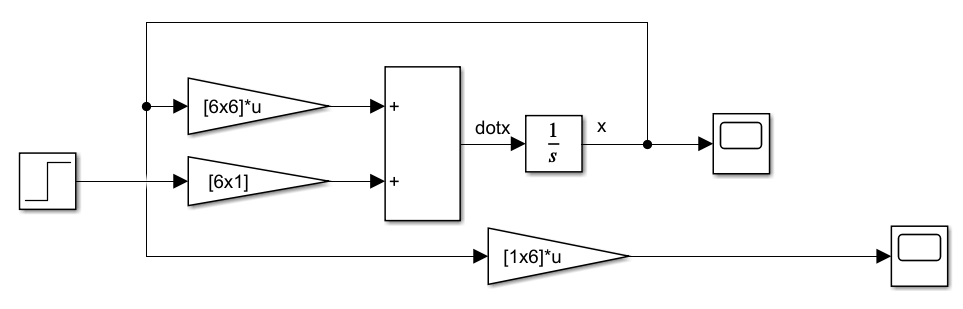
\includegraphics[width=.8\textwidth]{figure/exp1_1_model.png} 
%     \caption{Simulink模型} % caption是图片的标题
%     % \label{img} % 此处的label相当于一个图片的专属标志,目的是方便上下文的引用
% \end{figure}

% 导入代码
% \begin{lstlisting}
% a
% \end{lstlisting}

\begin{document}

\begin{titlepage}
% 封面信息
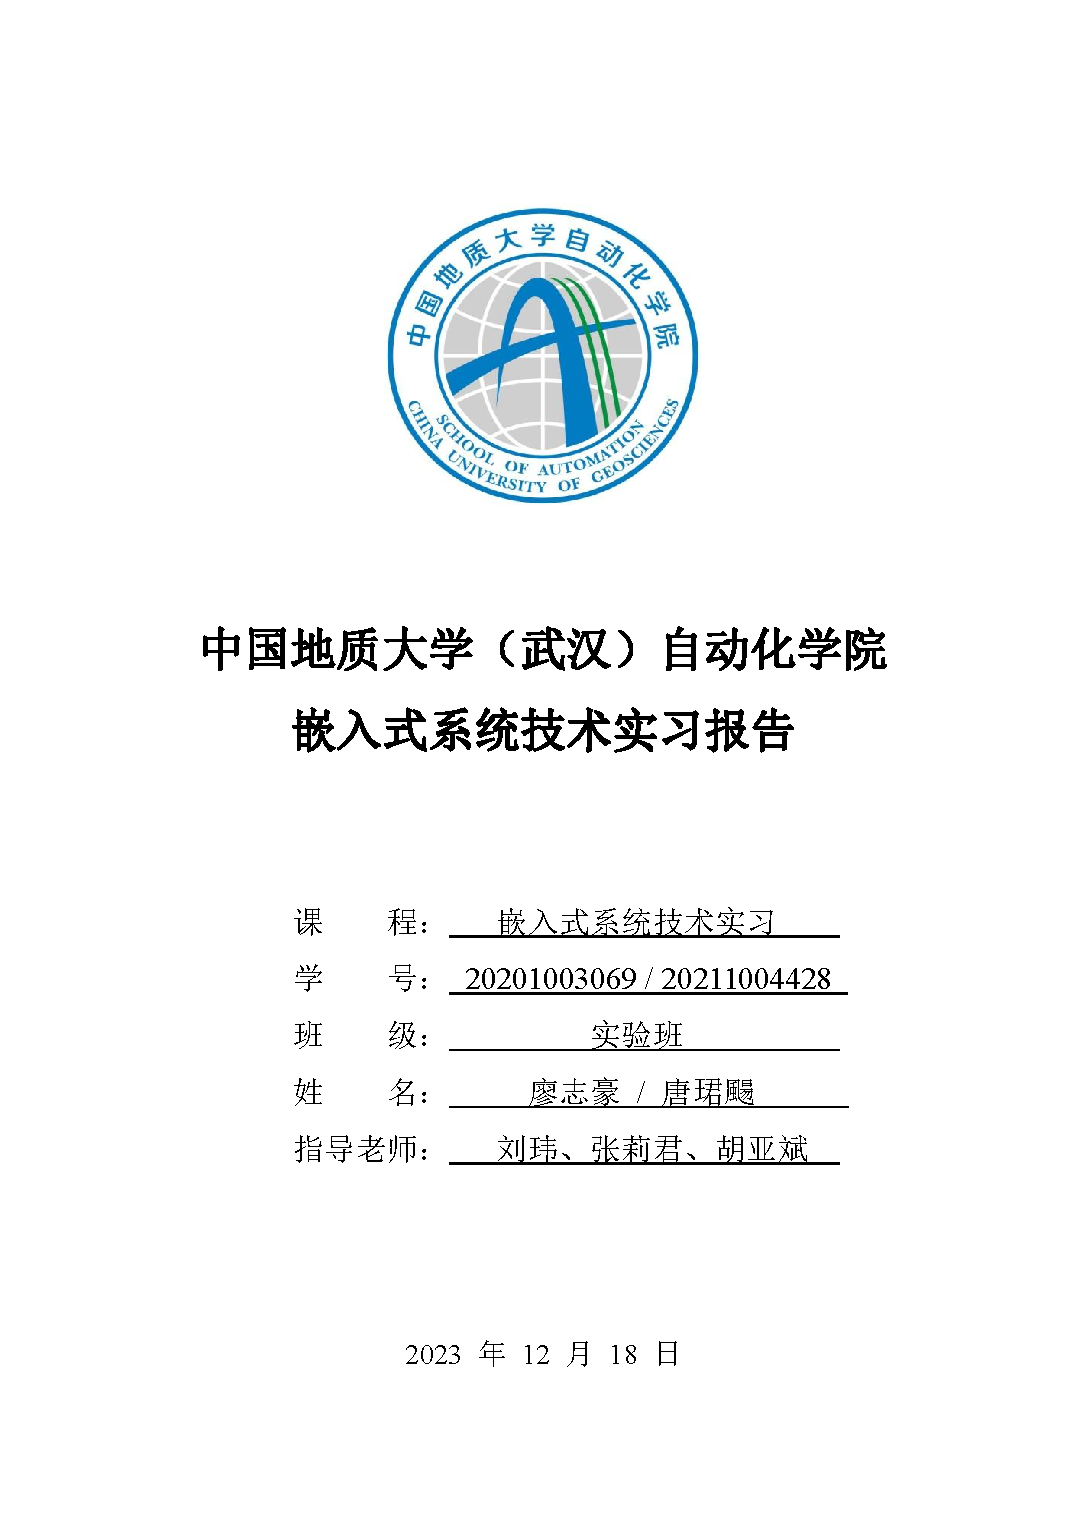
\includepdf[pages={1}]{cover.pdf}
\end{titlepage}

% 生成目录
\tableofcontents
\cleardoublepage

%
\section{第一部分:Jetson Nano开发板的探索}
% 内容:Jetson Nano开发板的硬件到软件模块的探索(例如:你所探索的硬件部件,Linux操作系统的熟悉使用,AI视觉算法模块的探究)
% 形式:一个部分的内容为一节;
% 目的:摸清每个探索过的模块
% 字数:不限(尽量详尽)

%%
\subsection{Jetson Nano开发板硬件与软件模块的探索}

%%%
\subsubsection{Linux操作系统Ubuntu的熟悉使用} 
%%%%
\paragraph{Ubuntu简介}~{}

Ubuntu是一个自由、开源、基于Debian的Linux操作系统,以友好的用户界面、强大的软件包管理器和广泛的社区支持而闻名。本次实习我们使用的Jetson Nano开发板自带的Linux镜像即为Ubuntu 18.04。

%%%%
\paragraph{系统换源}~{}

将Ubuntu系统的软件源更换为国内镜像源,可以大大提高下载和更新软件的速度。更换软件源的大致步骤如下:
\begin{enumerate}
    \item 备份原有的源文件。打开终端,输入命令:sudo cp /etc/apt/sources.list /etc/apt/sources.list.bak,即可完成备份。这样做的好处是,如果新的源不能使用或者出现其他问题,可以恢复原先的源。
    \item 备份完成后,在终端中输入命令:sudo nano /etc/apt/sources.list,打开源文件,删除所有现有内容,并添加新的软件源地址。推荐使用国内的镜像源,如清华镜像、阿里云、网易等,可以参考这些网站上对应版本的Ubuntu镜像源信息。
    \item 最后,保存并关闭文件,即可完成换源。
\end{enumerate}

%%%%
\paragraph{文件管理与命令行的使用}~{}

Linux文件系统:在Linux操作系统中,文件和目录是最基本的组织单位。与Windows操作系统不同,Linux操作系统采用树状结构来组织文件和目录。在Linux系统中,每个用户都有一个自己的主目录,通常位于/home/用户名/目录下。此外,Linux操作系统还有一些特殊的目录,如/bin、/sbin、/etc等,这些目录存放着系统的关键文件和程序。

命令行的使用:在Linux操作系统中,命令行是最常用的操作方式。通过输入特定的命令,用户可以完成对文件的操作,包括创建、删除、移动和重命名文件,以及系统配置、软件安装和使用等各种任务。

下面是一些常用的Linux命令:

\begin{table}[H] % 防止表格乱跑
\centering % 居中
\begin{tabular}{cc} % 指明列数
	\toprule % 顶部粗线
	命令 & 功能 \\
	\midrule % 中间细线
	pwd & 显示工作目录 \\
    cd & 切换工作目录 \\
    ls & 列出目录内容 \\
    touch & 创建文件 \\
    mkdir & 创建目录 \\
    cp & 复制文件或目录 \\
    mv & 移动或重命名现有的文件或目录 \\
    rm & 删除文件或目录 \\
	\bottomrule % 底部粗线
\end{tabular}
\caption{常用的Linux命令} % 标题
\end{table} 

此外,在不借助命令行的情况下,通过Ubuntu的图形界面也可以使用部分常用功能。

%%%%
\paragraph{软件安装与卸载}~{}

通过Ubuntu提供的命令行工具(如apt-get)可以非常容易地安装、更新和卸载软件。使用sudo apt-get install package\_name命令可以安装新的软件包,而sudo apt-get remove package\_name则可以卸载不需要的软件包。

用户也可以通过使用.deb文件进行软件的手动安装和卸载。在官网下载需要安装的软件的.deb文件,然后使用sudo dpkg -i package\_file.deb命令进行安装。如果需要卸载使用.deb文件安装的软件,可以使用sudo dpkg -r package\_name命令。此外,用户也可以通过Ubuntu的软件中心来管理软件的安装与卸载。

%%%%
\paragraph{远程访问}~{}

Ubuntu支持使用SSH客户端(如PuTTY)远程登录到Ubuntu系统,以及配置VNC服务器进行图形化远程桌面访问。由于在实习中我们直接使用显示器连接到开发板,因此没有对远程访问功能做深入研究,此处仅给出一些远程桌面连接相关的常用命令:

\begin{table}[H] % 防止表格乱跑
\centering % 居中
\begin{tabular}{cc} % 指明列数
    \toprule % 顶部粗线
    命令 & 功能 \\
    \midrule % 中间细线
    ping & 测试网络连通性 \\
    ifconfig & 查看和配置网络接口 \\
    netstat & 查看网络状态 \\
    ssh & 远程登录 \\
    \bottomrule % 底部粗线
\end{tabular}
\caption{远程桌面连接的常用命令} % 标题
\end{table} 

%%%%
\paragraph{其他}~{}

\begin{itemize}
    \item 在使用开发板时,Ubuntu系统可能会报如下错误:
    \begin{figure}[H]
    \centering % 居中 
    % 图片文件的相对路径
    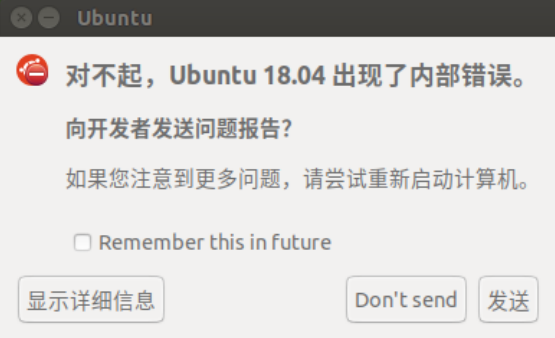
\includegraphics[width=.6\textwidth]{figure/系统报错.png} 
    \caption{Ubuntu系统报错} % caption是图片的标题
    % \label{img} % 此处的label相当于一个图片的专属标志,目的是方便上下文的引用
    \end{figure}
    然而系统并没有出现明显的故障和问题,在这种情况下,可以直接忽略该错误警告。(仅供参考)
    \item 在开发程序时,经常需要向开发板系统传输文件。然而我们在使用U盘时,遇到了系统提示挂载U盘失败的情况,使用网上提供的解决方案均无法解决问题,推测可能是U盘格式的问题。我们最后选择使用QQ实现远程文件传输。
\end{itemize}

%%%
\subsubsection{AI视觉算法} 
在针对AI视觉算法的学习中,我们先后探索了目标检测算法YOLOv5、物品检测模型SSD和著名的人脸识别开源项目face\_recognition。

%%%%
\paragraph{YOLOv5}~{}

% yolov5环境搭建和模型部署(花了大量时间,未成功)

YOLOv5,全称You Only Look Once version 5,是由Uitralytics公司发布的一种单阶段目标检测算法,它基于anchor来执行特征提取、融合、预测和优化的任务。这个模型在设计上采用了网格的概念,将图像划分为多个网格,每个网格负责预测一个或多个物体。这种网络结构的设计使用了全卷积网络和多尺度特征提取,使得每个网格都可以产生预测结果。在它的前一代YOLOv4的基础上,YOLOv5添加了一些新的改进思路,在速度与精度上都得到了极大的性能提升。

YOLOv5是本次实习我们最初选择的AI算法,我们计划使用该算法实现人脸识别功能。但是,在Jetson Nano开发板上为YOLOv5搭建环境时,我们遇到了很多棘手的问题。在这些问题上我们花费了大量的时间和精力,仍然没有得到妥善解决,最后我们不得不选择暂时搁置这个算法,转去研究别的项目。

%%%%
\paragraph{jetson-inference: 物品检测模型SSD}~{}

通过NVIDIA提供的jetson-inference推理框架,我们学习了物品检测模型SSD(Single Shot MultiBox Detector)。SSD是一种单阶段的目标检测算法,它在轻量级网络的基础上训练得到性能较优的模型。相比同为one-stage通用物体检测算法的YOLO,SSD的性能与速度要更优。

在对SSD模型的测试中,我们采集了58张人脸图像用于训练模型,训练后的模型可以成功检测到人脸。但是,由于SSD是一种物品检测模型,对于人脸检测的精度不高,且模型训练时间长,在之后的嵌入式系统设计中,我们没有采用SSD模型。以下是SSD模型的测试结果和运行数据:
\begin{figure}[H]
    \centering % 居中 
    % 图片文件的相对路径
    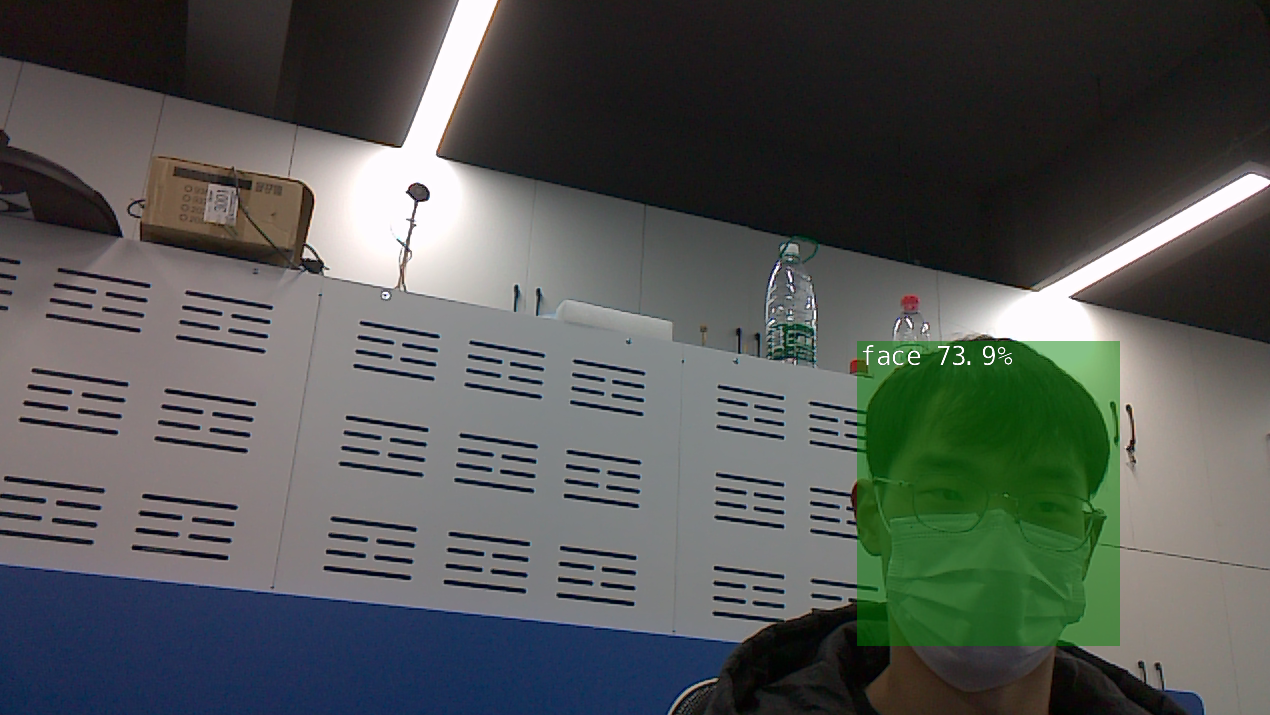
\includegraphics[width=.8\textwidth]{figure/ssd人脸识别效果.png} 
    \caption{SSD模型人脸识别效果} % caption是图片的标题
    % \label{img} % 此处的label相当于一个图片的专属标志,目的是方便上下文的引用
\end{figure}
\begin{figure}[H]
    \centering % 居中 
    % 图片文件的相对路径
    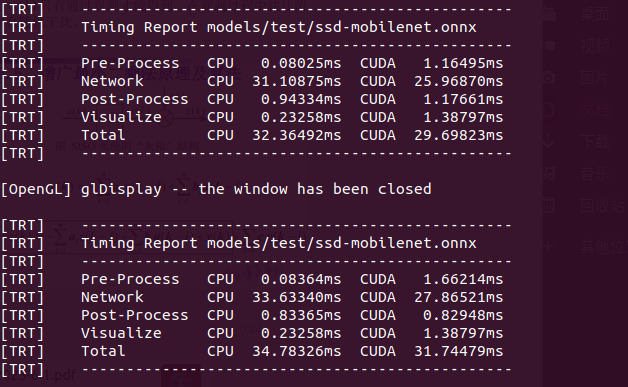
\includegraphics[width=.8\textwidth]{figure/ssd模型命令行运行信息.png} 
    \caption{SSD模型命令行运行信息} % caption是图片的标题
    % \label{img} % 此处的label相当于一个图片的专属标志,目的是方便上下文的引用
\end{figure}

%%%%
\paragraph{人脸检测:face\_recognition}~{}

face\_recognition人脸识别库是GitHub上的一个开源项目,基于业内领先的C++开源库dlib中的深度学习模型,专用于人脸识别,所需数据量少且识别精度高,非常适合用于嵌入式设备。

face\_recognition可以通过识别人脸关键点来检测图片中的人脸,并且采用特定的算法对人脸进行编码,使得可以将当前检测到的人脸对应的编码与已知人脸的编码进行对比,以获取当前人脸对应的具体身份信息。

基于face\_recognition提供的API,我们可以在图像中定位人脸位置、识别人脸关键点、获取图像中人的身份等。其常用的函数接口包括:
\begin{itemize}
    \item face\_encodings():对包含人脸的图像进行编码,获取人脸编码数据。
    \item compare\_faces():将待定的人脸编码与一组已知人脸编码数据进行比对,获取这些人脸编码是否匹配的信息。
    \item face\_distance():将一个已知人脸编码与一组人脸编码数据进行比对,获取这些人脸编码匹配程度的信息。
    \item face\_locations():识别图像中的人脸并获取其在图像中的位置信息。
\end{itemize}

%%%
\subsubsection{硬件部件} 
%%%%
\paragraph{Jetson.GPIO库}~{}

Jetson.GPIO库是专门为Jetson系列开发板设计的GPIO库,用于控制开发板上的通用输入输出引脚。它允许通过软件配置引脚的工作模式和输入输出状态,对引脚的电平进行读取或控制,并与其他设备进行交互。

Jetson Nano开发板基于Jetson.GPIO库可以实现中断(GPIO Interrupt)和事件(GPIO EVENT)。中断是将外部硬件设备上的状态变化连接到处理器的中断请求线上,触发中断时强制中断程序,事件在硬件级别上监听引脚变化,产生中断信号。

此外,Jetson Nano不支持直接输出 PWM 波,如有需要可以考虑外接I2C转PWM信号的模块来实现 PWM 波输出。

% \paragraph{UART/I2C通信}~{} 

% pySMbus 库:pySMbus 库是一个通过 Python 控制 I2C 设备的常用工具,是一种简化版本的 I2C 总线,smbus库是标准库的一部分,不需要额外安装。可以通过库中的函数向设备寄存器中发送和从设备寄存器中读取字节数据,可以通过这些函数与外部设备进行 I2C 通信。
% -- pySerial
% --- pySerial 库是 python 的一个串口通信库,支持不同平台的串口操作,可以非常方便的实现对串口进行读写操作。
% --- 在进行串口通信时,应该注意外接设备的电平状态,可能需要外接适当的适配器或者电平转换器,在进行物理连接时注意采取相应的物理和逻辑保护措施,保证通信的平稳和设备的安全。


\paragraph{CSI摄像头}~{}

在探索Jetson Nano开发板的过程中,我们在摄像头的调用上遇到了各种问题,以下是我们尝试过的方法、遇到的问题以及部分解决思路:
\begin{itemize}
    \item 计算机视觉库OpenCV-Python 
    
    遇到的问题:我们在尝试使用OpenCV-Python打开摄像头时总是出现报错,通过查阅相关资料我们认为可能是因为使用的jetson nano开发板自带的系统镜像中,OpenCV-Python库的版本和现有的Python版本不匹配。

    可能的解决思路:经过研究发现,Jetson Nano开发板自带的镜像系统中包含两个Python版本:Python2.7.17和Python3.6.9,这两个Python版本下各自附带有一个OpenCV-Python软件包,分别是OpenCV-Python4.1.1和OpenCV-Python3.2.0。

    经过测试我们发现,Python3下OpenCV的版本较低,无法成功调用摄像头;Python2下OpenCV可以成功调用摄像头。但是考虑到之后程序的兼容问题,我们放弃使用Python2版本。

    之后我们尝试升级OpenCV的版本,没有成功,通过查阅资料我们发现,Jetson Nano开发板下无法通过软件包镜像文件(.whl)的方式直接安装OpenCV(我们没有找到与Jetson Nano开发板ubuntu系统匹配的镜像文件),因而只能通过源代码编译的方式进行安装,但是这种方式耗时非常长而且失败率高,最后我们没有采用,但它仍不失为一个可行的解决方案。

    \item JetCam
    
    JetCam是用于NVIDIA Jetson的易于使用的Python相机界面。使用Jetson的Accelerated GStreamer插件可与各种USB和CSI摄像机配合使用。能够读取图像数据作为numpy数组,便于进行图像处理。

    我们发现,Jetson Nano开发板的镜像系统中已经安装了jetcam,然而我们在尝试使用jetcam调用摄像头读取视频数据时报错,摄像头无法成功初始化。考虑到可能是由于开发板自带镜像系统中部分文件不全,我们尝试重新安装了一遍jetcam,仍然无法解决该问题,最后放弃了这个方案。

    \item nvgstcapture gstreamer应用程序
        
    nvgstcapture是一个由NVIDIA提供的命令行工具,主要用于在NVIDIA Jetson平台上进行视频捕获。它是一个基于GStreamer的应用程序,可以用于实时捕获视频流并将其保存为文件。由于该程序需要在命令行中调用,因此我们还使用了Python下的subprocess模块在python程序中调用该命令,成功实现了摄像头的调用以及图像数据采集。但是在后来嵌入式系统的开发过程中,我们觉得这种调用方式过于繁琐,而且nvgstcapture命令行工具给出的功能十分有限,因此我们最后选择了另一种方式:jetson.utils。

    \item jetson.utils
    
    jetson.utils是为了方便开发人员使用Jeston设备而开发的Python库,提供了很多实用的功能接口。这个库由NVIDIA的工程师在GitHub上开源。
    (见\url{https://github.com/dusty-nv/jetson-utils})

    最终采用的摄像头调用方案:使用jetson.utils库实现视频流读取和转OpenCV图像。我们使用jetson.utils库对摄像头进行调用,以获取图像数据。对于后续的图像处理等任务,则使用OpenCV-Python来进行。

    需要注意的地方:在使用jetson.utils库的过程中,我们通过在网上查找资料发现,由于jetson.utils库通常是作为jetson-inference项目的子模块构建的,因此导致在使用jetson.utils库过程中遇到的问题,以及jetson.utils库的一些使用方法,在jetson.utils的GitHub项目中无法找到,而要去jetson-inference的GitHub项目中寻找。
    
\end{itemize}

%%%%
\paragraph{对开发板上GPU的探索}~{}

Jetson Nano 开发板上搭载了一块128核Maxwell GPU,不仅可以用于加速图形处理,还可以用于加速深度学习推理任务。通过使用 NVIDIA 提供的软件工具(如 TensorRT 和 CUDA),开发者可以利用 GPU 在 Jetson Nano 上高效地执行深度学习模型推理任务。

% 在对AI视觉算法YOLOv5探索的过程中,我们对CUDA和TensorRT进行了一些了解。

CUDA:CUDA 是 NVIDIA 推出的一种通用并行计算平台和编程模型。它允许开发者使用 C 或 C++ 语言来编写并行计算程序,以在NVIDIA 的 GPU(图形处理器)上进行高性能计算。CUDA 提供了一套 API 和工具,用于管理和执行 GPU 上的并行计算任务。GPU在并行计算方面具有很高的性能和处理能力。CUDA利用GPU上的大量并行计算单元(CUDA核心)和内存带宽,能够加速各种计算密集型应用程序,包括科学计算、机器学习、图像处理等。CUDA 通过调用定义和调用核函数的方式启动 GPU 的线程块,并在 GPU 上启动这些线程,在线程执行结束之后 CUDA 将核函数结果复制回主机,并对内存进行清理。

TensorRT:TensorRT 是由 NVIDIA 开发的深度学习推理(inference)优化器和运行时引擎。它可以将经过训练的深度学习模型转换为高效的、针对特定硬件架构优化的推理引擎,从而实现更快速且低延迟的推理性能。TensorRT 支持各种深度学习框架训练的模型,如TensorFlow、PyTorch、Caffe 等。它提供了一系列的 C++ 和Python API,以及用于模型优化和部署的工具,简化了模型优化和推理部署的过程。



%%
\subsection{实习心得}
%%%
\subsubsection{遇到问题及解决} 

% 探索期间遇到的问题
开发板的镜像系统中项目文件不全:对于本次实习提供的Jetson Nano开发板,亚博智能官方网站给出了一些针对AI视觉的学习教程,并且开发板自带的镜像系统中附带了教程内容中涉及到的部分AI模型项目文件。但是,这些模型有一部分无法成功运行,因为其中的一些文件存在缺失或损坏。后来我们在和其他同学的交流中得知,这些模型可以在NVIDIA的GitHub项目jetson-inference中找到。

环境搭建中软件包无法使用和版本不匹配的问题:我们在尝试为YOLOv5等项目搭建实验环境时发现,由于某些尚不清楚的原因,镜像系统中附带的一些软件包无法正常使用。遇到这种情况,可以尝试将软件包卸载以后重新安装。此外,Python下的环境搭建对于包版本的要求比较严格,在安装时需要仔细甄别项目的需求,盲目安装最新版本可能导致最后环境无法使用。

%%%
\subsubsection{收获与感想} %(必写内容)
学习路线陡峭:本次基于Jetson Nano开发板的嵌入式系统开发涉及到的知识面较广,不仅要熟练掌握课程所教授的Linux操作系统方面的知识,而且要自主学习一些新的东西,如Python语言的学习和使用,嵌入式AI算法的环境搭建和部署等。因此,要想掌握嵌入式开发,需要付出大量的时间和精力去学习和实践,这也让我们更加珍惜所学到的每一项技能。

动手实践的重要性:嵌入式是一门实践性很强的学科,理论知识的学习只是基础。在实习过程中,我们通过动手搭建Jetson Nano开发环境、编写程序、调试硬件等方式,将所学的理论知识应用到实际项目中。这种实践过程让我们更加深入地理解了嵌入式系统的工作原理,也锻炼了我们的动手能力和解决问题的能力。

耐心和毅力:在实习过程中,我们遇到了很多困难和挑战。面对这些问题,保持耐心和毅力是非常重要的,只有不断地尝试和改进才能获得成功。有时候,一个问题可能需要花费很长时间才能解决,但正是这种坚持不懈的精神,让我们在实习过程中取得了很大的进步。

%%
\subsection{思考并回答以下问题}
%%%
\subsubsection{Jetson Nano这套板子与实验所用的板子的异同有哪些?} 
%%%%
\paragraph{相同之处}~{}

Jetson Nano开发板和S3C2440开发板都是嵌入式开发板,且都属于ARM架构,在基本的硬件接口上也有相似的地方,如USB、网口等。

\paragraph{不同之处}~{}

\noindent Jetson Nano:
\begin{itemize}
    \item 性能更高,可以比较流畅地运行Ubuntu18.04操作系统,可以在本机直接进行软件开发,操作更加方便。
    \item Jetson Nano所搭载的硬件资源更多,配置更高,可以支持许多流行的深度学习框架,如TensorFlow、PyTorch等。适用于人工智能、机器人、自动驾驶、医疗和安防等领域的开发和应用。
    \item 在硬件配置上,包含了一块128核Maxwell架构的GPU,在体积上采用核心板可拆的设计,核心板的大小只有70 x 45 mm,可以很方便地集成在各种嵌入式应用中。同时它的功耗也非常低(低功耗模式5W,10W模式下需在散热片上安装风扇以防止死机)。
\end{itemize}

% 处理器和GPU: Jetson Nano搭载四核Cortex-A57处理器和128核Maxwell GPU,
% 内存: Jetson Nano具有4GB LPDDR内存,可支持深度学习和其他高带宽应用。

\noindent 实验所用开发板TQ2440:
\begin{itemize}
    \item 开发过程比较繁琐,需要利用上位机进行代码的编写和程序烧录调试,接线比较麻烦(需要连接一根烧录线,一根串口通信线以及一根串口转USB线)。
    \item 和Jetson Nano开发板相比,硬件配置比较老旧,性能不高,在软件方面的支持相对较少。更多地用于一般的嵌入式应用,适用领域相对受限。
    \item 在硬件配置上,其CPU为ARM Cortex-A9内核,底板搭载了常用的外设扩展和接口,如存储器芯片(分为3种:SDRAM,NOR FLASH,NAND FLASH),音频输入输出接口,USB接口,串口,Jtag,LCD显示屏等。
\end{itemize}

%%%
\subsubsection{本开发板基于Linux之上开发AI算法,对底层硬件需要了解吗?} 

在使用Jetson Nano开发板进行基于Linux的AI算法开发时,对底层硬件的了解是有一定帮助的。

Jetson Nano作为一款可应用于人工智能的嵌入式开发板,体积小巧但功能强大,搭载了四核ARM Cortex-A57处理器和NVIDIA研发的128核Maxwell GPU,并且提供了摄像头,USB等众多外设扩展和接口,还具有低功耗的特性。因此,了解其硬件配置、参数、性能和使用方法等基本信息,可以帮助开发者更好地发挥出该开发板的性能优势。

Jetson Nano开发板提供了两个CSI摄像头接口,可以实时处理多个高清全动态视频流。在进行有关视频图像处理的AI算法开发时,了解摄像头等相关硬件的调用方式和底层程序运行逻辑是非常有必要的。同时对于大多数AI项目来说,往往需要涉及到大量的计算任务,或者存在着多任务并行计算的需求,那么在针对这些计算任务的加速计算和优化处理的过程中,也需要开发者对于开发板底层硬件的支持情况有一定的了解。此外,通常AI算法对于算力的要求较高,需要对开发板所搭载的计算资源有一定的了解,以评估该开发板适合运行的AI算法。

然而,虽然对硬件有所了解可以带来一定的好处,但对于大部分基于Linux的AI算法开发来说,并不需要特别深入地了解硬件层面的内容。因为Jetson Nano开发板预装了Ubuntu 18.04LTS(长期支持版本)操作系统,在硬件调用上有着更加完备的支持,同时还提供了丰富的软件支持和API接口,使得开发者可以在不深入了解底层硬件的情况下进行软件开发。值得一提的是,Jetson Nano的用户界面也相当友好,有利于新手的快速入门。

总的来说,对Jetson Nano底层硬件的了解可以帮助开发者更好地利用其性能优势和特点,但对于大部分基于Linux的AI算法开发来说,并不是必须的。主要的开发工作仍然主要集中在算法设计和实现上。

%%%
\subsubsection{如果前期对ARM硬件有一定的了解,对Linux之上的开发有帮助吗?帮助在哪里?} 
对ARM硬件有一定了解可以为Linux上的开发提供帮助:
\begin{itemize}
    \item 理解ARM架构和其特性可以帮助开发者更好地理解硬件如何与软件进行交互。这将使开发者能够更有效地利用硬件资源,例如处理器、内存和外设。
    \item 了解ARM架构也有助于开发者理解Jetson Nano的硬件配置和性能特点。这包括对GPU架构的理解,以及对内存管理和电源供应方式的了解。这些知识可以帮助开发者在进行AI算法开发时,更好地优化性能并解决可能出现的问题。
    \item 掌握ARM基础知识有助于开发者更好地使用和理解Jetson Nano提供的软件开发工具和接口。例如,对于需要在多个高清视频流上实时处理的AI应用,了解ARM的并行处理能力将非常有帮助。
\end{itemize}


%
\section{第二部分:嵌入式系统设计及实现--基于人脸识别的智能门锁与监控系统}
% 内容:设计的嵌入式应用系统
% 形式:不限;
% 目的:讲清楚自己的系统,如何设计,如何实现
% 字数:不限

%%
\subsection{系统设计及实现}
%%%
\subsubsection{系统介绍} 
基于人脸识别的智能门锁与监控系统:

%%%%
\paragraph{实现的功能}~{}

人脸注册功能:用户输入姓名,并采集一张包含完整脸部特征的图片即可完成人脸注册;若采集到的图片信息有误系统将给出提示信息。

人脸实时识别功能:可以实时识别视野中的所有人脸,并标记出已注册的人脸(显示姓名)和未注册的人脸(提示“Unknown”)。

设计了ui界面,包含人脸采集模块和人脸实时识别模块,方便用户使用。

%%%%
\paragraph{有待完善的功能}~{}
\begin{enumerate}
    \item 基于Jetson.GPIO,实现开发板对外设(门锁)的控制。
    \item 开发板与其他设备或模块(如小型LCD显示屏)的通信。
    \item 人机交互部分功能扩展。
\end{enumerate}

%%%%
\paragraph{设想的使用场景}~{}

基于人脸识别的门锁:使用者注册自己的人脸后,系统在检测到使用者的脸部特征时即可为使用者开门。

智能监控:系统可以记录检测到的人脸,并记录检测时间等信息,方便使用者查看是否有可疑人员在门外驻留。

%%%
\subsubsection{系统实现} 
%%%%
\paragraph{UI界面}~{}

本次开发的基于人脸识别的智能门锁与监控系统提供了一个面向用户的简易ui界面,主要包含两大功能模块,分别提供人脸信息注册功能和人脸实时识别功能,界面设计如下所示:
\begin{figure}[H]
    \centering % 居中 
    % 图片文件的相对路径
    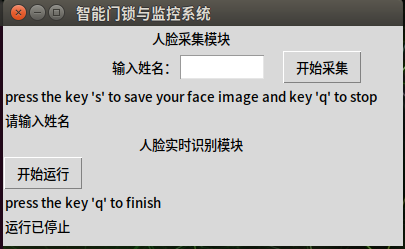
\includegraphics[width=.6\textwidth]{figure/ui界面.png} 
    \caption{UI界面设计} % caption是图片的标题
    % \label{img} % 此处的label相当于一个图片的专属标志,目的是方便上下文的引用
\end{figure}

该UI界面基于Tkinter(tk interface)开发。Tkinter是Python自带的标准GUI库,无需另行安装,支持跨平台运行,支持的操作系统包括Windows、Linux和Mac等。相比于通常的图形化界面开发工具PyQt,Tkinter更加轻量,更适合在嵌入式系统的开发中使用;但是在性能和功能的丰富程度上Tkinter相对较差,只适合开发一些简单的程序。综合考虑我们选择使用Tkinter来进行UI界面的开发。


% - 功能实现
% 考虑到系统的内存空间限制,我们使用vscode作为开发工具用于代码编辑,在命令行进行代码的编译和运行。

\paragraph{摄像头调用和图像处理}~{}

使用jetson.utils工具可以实现对CSI摄像头图像数据的读取,使用videoSource()函数以创建一个视频流对象:
\begin{lstlisting}
# 读取视频流
input_video = jetson.utils.videoSource("csi://0") 
\end{lstlisting}

通过调用该对象的Capture()函数可以获取摄像头当前捕获的一张图片:
\begin{lstlisting}
utils_img = input_video.Capture()
\end{lstlisting}

此时获取的图像为utils库使用的格式,要想正常使用OpenCV-Python处理这些图片,还需要将格式转为OpenCV-Python可以处理的BGR格式:
\begin{figure}[H]
    \centering % 居中 
    % 图片文件的相对路径
    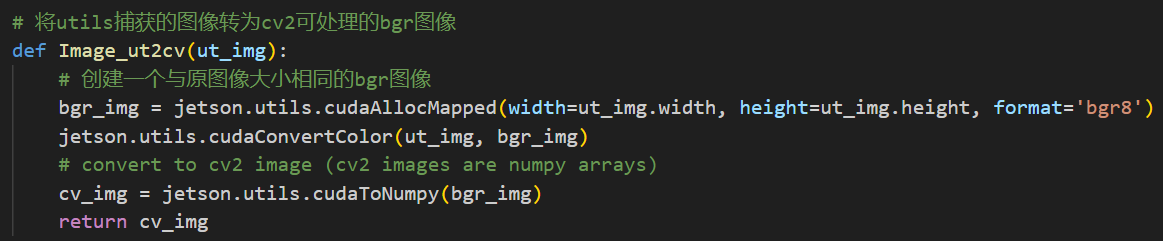
\includegraphics[width=1\textwidth]{figure/ut2cv.png} 
    % \label{img} % 此处的label相当于一个图片的专属标志,目的是方便上下文的引用
\end{figure}

要在窗口中显示图像,可以通过jetson.utils的videoOutput()函数,创建一个视频流输出对象,并调用其屏幕输出函数Render():
\begin{lstlisting}
# 创建一个视频流输出对象
output = jetson.utils.videoOutput("display://0")
# 指定屏幕输出
output.Render(img)
\end{lstlisting}

在我们设计的系统中,由于需要OpenCV-Python来进行图像处理,因此使用cv2下的屏幕输出函数:
\begin{lstlisting}
cv2.imshow("face register", cv_img)
\end{lstlisting}

此外,在系统的实现中,我们还使用cv2来进行图像的格式转换、压缩、绘制元素、图像读取和保存、按键检测等处理任务。

%%%%
\paragraph{人脸识别:face\_recognition}~{}

在本系统的开发中,我们主要使用face\_recognition来实现人脸的检测与身份识别。face\_recognition可以通过识别人脸关键点来检测图片中的人脸,并且采用特定的算法对人脸进行编码,使得可以将当前检测到的人脸对应的编码与已知人脸的编码进行对比,以获取当前人脸对应的具体身份信息。

基于face\_recognition提供的API,我们可以在图像中定位人脸位置、识别人脸关键点、获取图像中人的身份等。其常用的函数接口包括:
\begin{itemize}
    \item face\_encodings():对包含人脸的图像进行编码,获取人脸编码数据。
    \item compare\_faces():将待定的人脸编码与一组已知人脸编码数据进行比对,获取这些人脸编码是否匹配的信息。
    \item face\_distance():将一个已知人脸编码与一组人脸编码数据进行比对,获取这些人脸编码匹配程度的信息。
    \item face\_locations():识别图像中的人脸并获取其在图像中的位置信息。
\end{itemize}

由于face\_recognition处理的图像为RGB格式,因此在进行人脸识别之前,需要对获取的图像进行格式转换;此外,为了提高处理速度,我们还可以对图像进行适当的压缩:
\begin{figure}[H]
    \centering % 居中 
    % 图片文件的相对路径
    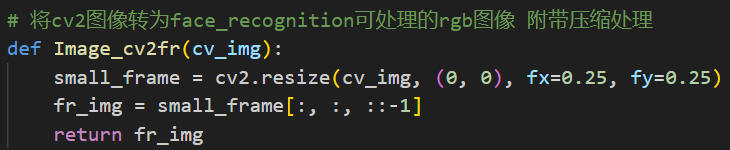
\includegraphics[width=1\textwidth]{figure/cv2fr.png} 
    % \label{img} % 此处的label相当于一个图片的专属标志,目的是方便上下文的引用
\end{figure}

%%%%
\paragraph{人脸信息登记}~{}

人脸信息登记功能要求用户首先在UI界面中输入待注册的人的姓名,输入完成后点击“开始采集”按键即可开启摄像头进行图像采集。用户可以根据界面中的提示,点击特定按键后,系统即捕获当前的图像并对其进行人脸检测。为了防止系统在运行中出现不必要的错误,此处对于采集到的人脸图像设定了较为严格的要求:图像中只能出现一个有效的人脸,以便于对人脸的面部特征进行编码以及匹配其身份信息。当采集到的人脸图像不符合要求时,系统将会给出提示信息(“人脸信息采集失败,请重试”);在人脸图像采集完成后,系统也将给出提示(“人脸信息采集成功”)。

此外,系统对于采集到的人脸信息,专门建立了一个文件夹用于存放人脸图像。在开启人脸实时识别功能时,系统可能会访问该文件以加载需要的注册信息。

%%%%
\paragraph{实时人脸识别}~{}

实时人脸识别功能的大致思路是,对于当前捕获的一帧图像,识别出其中的所有人脸并获得其对应的人脸编码。将这些身份信息待定的人脸编码与系统中保存的已知人脸编码数据进行对比,若待定的人脸编码在已知数据库中存在匹配度较高的对应编码,则可以获取其身份信息,系统会在监控窗口中用绿色方框框出该人脸并标识出对应的身份信息(即姓名);若无法找到匹配的编码,则认为其身份信息未知,将该人脸在监控窗口中用红色方框框出,并标识为未知("Unknown")。

在运行实时人脸识别之前,系统需要首先加载已经注册的人脸信息,即人脸编码以及对应的身份信息(姓名):
\begin{figure}[H]
    \centering % 居中 
    % 图片文件的相对路径
    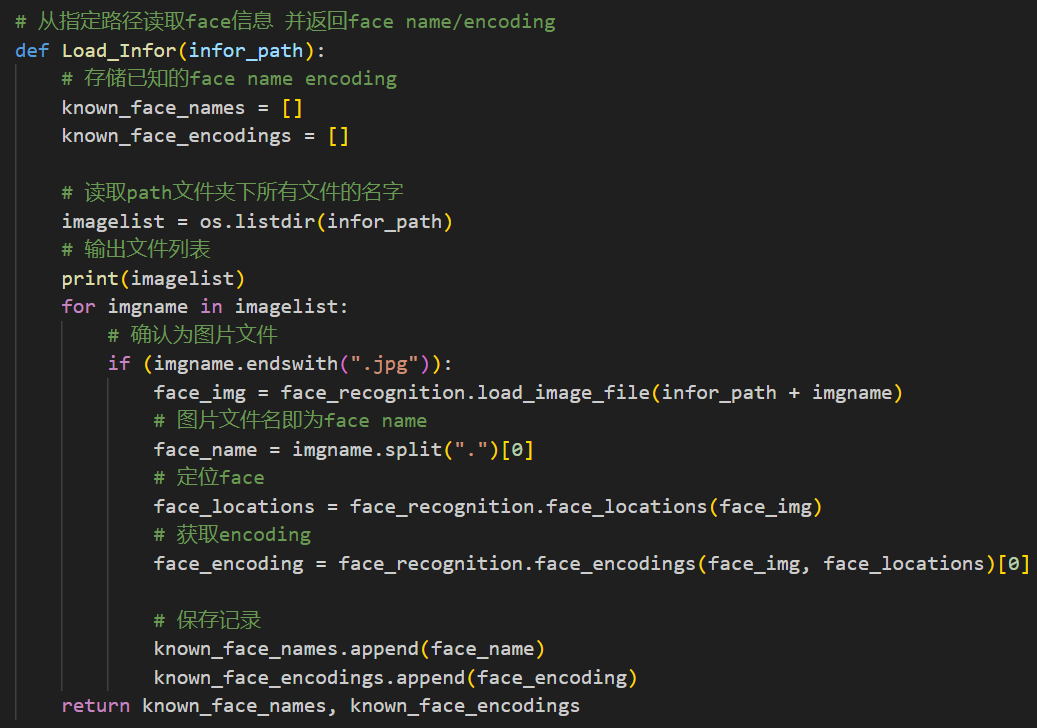
\includegraphics[width=1\textwidth]{figure/load_infor.png} 
    % \label{img} % 此处的label相当于一个图片的专属标志,目的是方便上下文的引用
\end{figure}
对于系统具体实现的其他细节,可以参考附录中的源代码。

%%%
\subsubsection{测试效果展示} 
测试使用的数据集如下:
\begin{figure}[H]
    \centering % 居中 
    % 图片文件的相对路径
    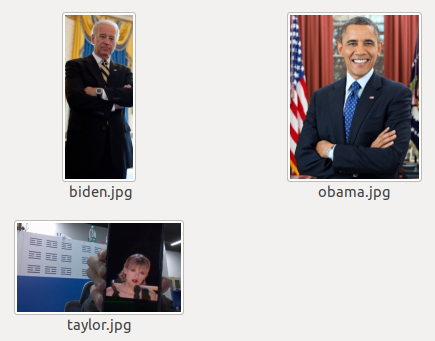
\includegraphics[width=.6\textwidth]{figure/数据集.png} 
    \caption{测试数据集} % caption是图片的标题
    % \label{img} % 此处的label相当于一个图片的专属标志,目的是方便上下文的引用
\end{figure}
数据集图像中的人物分别是Biden(年老),Obama,Taylor。其识别结果如下:
\begin{figure}[htbp]
	\centering
	\begin{minipage}{0.49\linewidth}
		\centering
		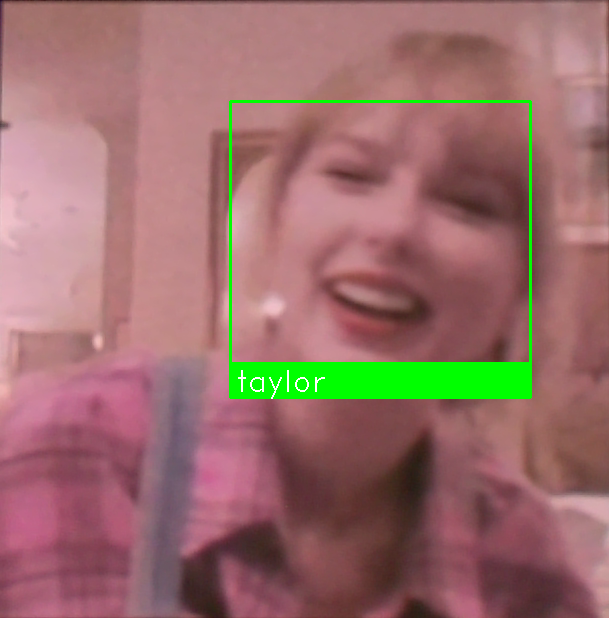
\includegraphics[width=0.9\linewidth]{figure/效果展示.png}
		\caption{Taylor}
		% \label{chutian1}%文中引用该图片代号
	\end{minipage}
	%\qquad
	\begin{minipage}{0.49\linewidth}
		\centering
		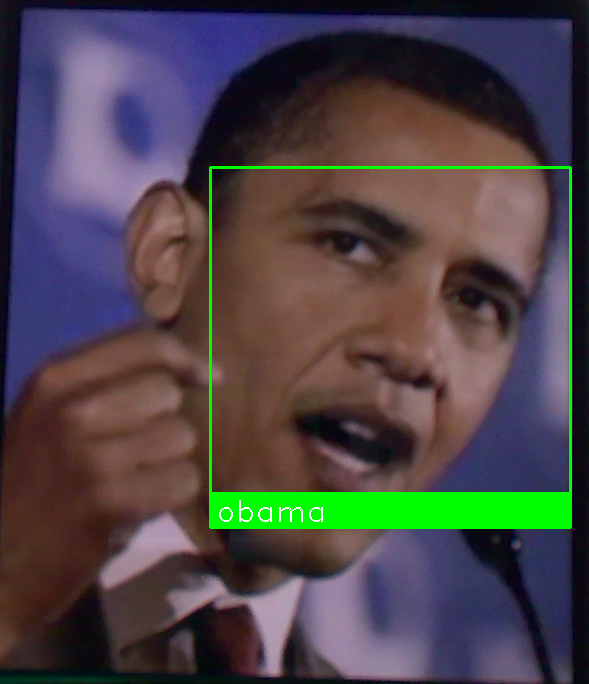
\includegraphics[width=0.8\linewidth]{figure/效果展示3.png}
		\caption{Obama}
		% \label{chutian2}%文中引用该图片代号
	\end{minipage}
\end{figure}
\begin{figure}[H]
    \centering % 居中 
    % 图片文件的相对路径
    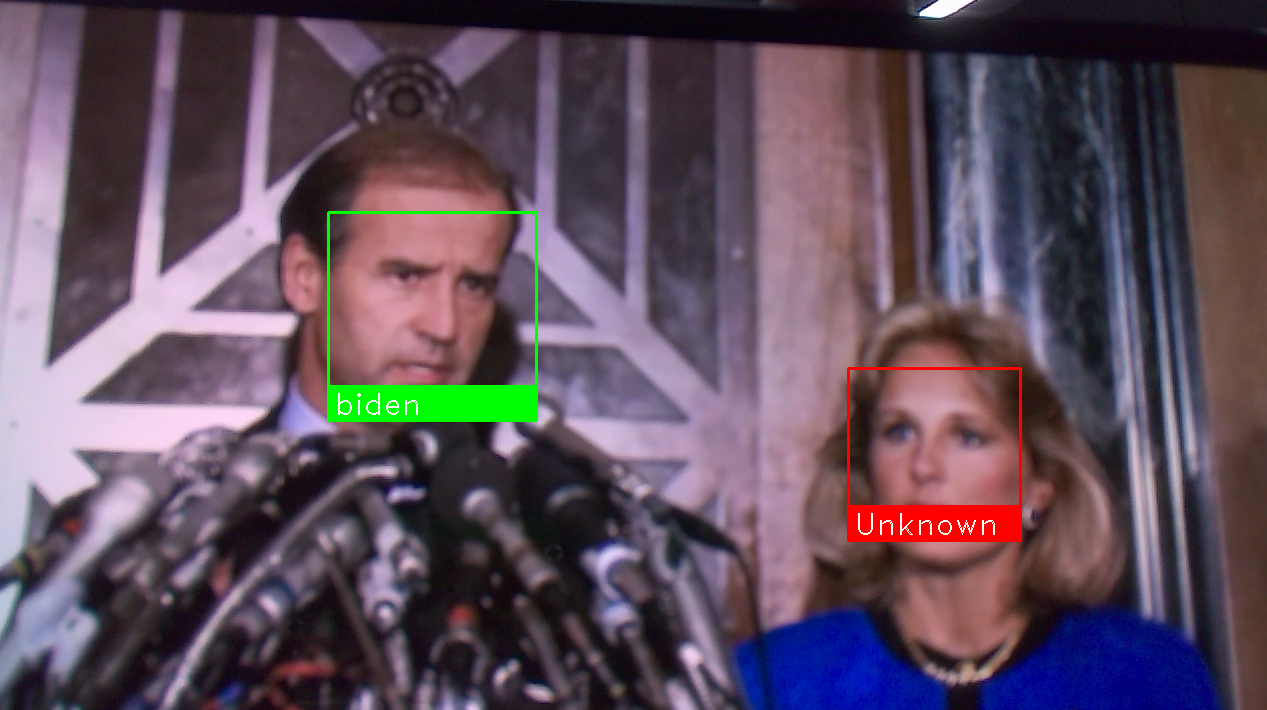
\includegraphics[width=.6\textwidth]{figure/效果展示2.png} 
    \caption{Biden(年轻)} % caption是图片的标题
    % \label{img} % 此处的label相当于一个图片的专属标志,目的是方便上下文的引用
\end{figure}
由测试结果可以看到,系统在视野较模糊(与背景区分度不大)的情况仍可以准确识别到人脸;且对于同一个人,其年轻和年老的样貌变化对于识别结果的影响不大,说明该系统的识别精度高,适用性较强。

%%
\subsection{实习心得}
%%%
\subsubsection{遇到问题及解决}
% 嵌入式系统开发过程中遇到的问题
AI算法的环境搭建和部署:在本次实习中,我们遇到的一个非常棘手的问题就是对AI算法的环境搭建和部署。最初我们选择YOLOv5项目作为学习对象,但是在为它搭建环境时遇到了很多问题,最后由于时间耗费太多我们不得不放弃这个AI算法。

%%%
\subsubsection{收获与感想} %(必写内容)
% - 团队协作与沟通
% - 创新思维的培养
% - 嵌入式开发流程的学习和了解
% - 兴趣

%%%%
\paragraph{团队协作与沟通}~{}

本次实习以两人为一组共用一台设备,这就要求小组的每个成员要有相对明确的分工和合作。在实习过程中我们小组首先经过讨论得出了一个大致的设计目标和学习计划,分不同的方向来进行学习和项目复现等工作。通过这种分工协作的方式,我们在学习了各自感兴趣的技术的同时也共同解决了许多问题,最后相对顺利地完成了本次实习的要求。

不仅如此,在整个实习的过程中,小组之间的交流和互相学习也是非常重要的一个方面。我们和其他小组的同学在线上和线下都有一些非常具有帮助和启发意义的讨论,在这些相互之间不断沟通交流和分享经验的过程中,我们也学习到了很多解决问题的有效思路和面对疑难问题的应对方式。这样既培养了团队内成员的协作能力,又锻炼了团队之间的沟通能力。

%%%%
\paragraph{嵌入式开发流程的学习和了解}~{}

在实习中,我们通过自主学习深入了解了嵌入式开发的基本流程。首先要明确任务需求,基于需求来确定系统的设计方案,包括软件开发所需工具和硬件配置的要求,然后进行系统的软硬件开发,最后是针对系统的调试、验证和修改,直到系统满足我们的需求,最后完成嵌入式系统的部署工作。

%%%%
\paragraph{创新思维的培养}~{}

本次实习并没有给出特别明确的实习任务和实习目标。我们小组在初期经过讨论决定,以人脸识别等AI算法作为切入点,基于官方提供的教程和资料,以及在CSDN、GitHub等开源平台和学习论坛中获取的相关参考资料和学习资源,进行Jetson Nano开发板的探索以及AI算法的学习和部署。在对开发板的探索和学习过程中,我们基于现有开源算法进行创新,设计并实现了一个综合性的嵌入式系统,极大地提升了自身的学习能力和创新能力。

%%%%
\paragraph{兴趣的培养}~{}

兴趣是最好的老师,在实习中我们出于对AI算法的浓厚兴趣,自主学习了很多相关知识。结合目前正在学习的《人工智能基础》课程,我们查阅了一些人工智能算法方面的资料,对于人工智能背后的原理有了更深刻的认识。此外,我们小组对于以Ubuntu为代表的Linux操作系统也产生了一定的兴趣,其基于命令行的工作模式,以及Linux操作系统下的软件生态对于提高软件开发效率等方面非常有帮助,可以考虑将Linux融入到我们的日常学习和工作中。


%%
\subsection{思考以下问题并回答}
%%%
\subsubsection{你感觉开发板与嵌入式课程的联系有哪些?} 
开发板的使用基于Linux操作系统Ubuntu,可以进一步加深对Linux操作系统、文件系统和命令行工具的理解和熟悉。

基于Ubuntu操作系统下的AI项目开发,会部分涉及到驱动程序的开发和使用,如GPIO等。此外,还会涉及到ARM嵌入式系统的相关硬件知识,如外围电路(时钟和电源管理,系统复位,存储器扩展)和接口电路(串口,USB,GPIO端口,HDMI,网口)等。这些都是对嵌入式课程内容的补充和扩展。



%%%
\subsubsection{Jetson Nano是否适合拿来作为实习用?为什么?} 
我认为Jetson Nano开发板非常适合作为嵌入式课程实习用的工具。理由如下:
\begin{itemize}
    \item 在通过使用Jetson Nano开发板进行基于Linux操作系统的AI算法开发时,可以学习到很多有关Linux操作系统实际使用方面的相关知识,而且可以对嵌入式应用系统开发流程有更全面的了解,也更贴近当前主流的嵌入式系统开发方式。
    \item Jetson Nano作为一款体积小巧且功能强大的人工智能嵌入式开发板,它的可玩性非常高,能够在它之上开发各种各样的基于AI的嵌入式应用系统。这样可以非常好地激发学生的学习探索兴趣以及创新思维和动手能力,在实践中深入理解和体会嵌入式系统与当前流行的人工智能技术之间的内在联系和应用价值。
    \item 随着现在人工智能技术的迅速发展,在未来各种AI算法将会更多地结合到嵌入式应用系统中。而Jetson Nano开发板作为一款性能相对优秀的边缘AI计算设备,可以很好地帮助学生掌握将人工智能技术与嵌入式系统两者相结合的相关知识和技能,比如在嵌入式开发过程中增加深度学习的功能、在嵌入式应用系统中部署AI算法和模型等。而且这款开发套件基于Linux开源操作系统,其背后的开发者社区支持是非常完备的。
    \item 此外,利用Jetson Nano开发板完成嵌入式实习还可以促使学生掌握更多的其它相关技术和技能。比如大部分AI算法的学习和使用都需要一定的python基础,虽然可能需要一定的时间学习,但python语言本身十分简单,容易上手,且应用非常广泛,是一个学习新知识的好机会。
\end{itemize}

综上所述,我认为Jetson Nano开发板能够极大地丰富嵌入式实习课程的教学内容和形式,激发学生的学习兴趣,达到更好的学习效果。

%%%
\subsubsection{有哪些内容是你希望老师在课堂上教授的?} 
有关开发板的基础知识和基本使用方法:硬件资源和配置,包括GPU和CPU运算平台的基本信息如架构、技术规格和内存等具体参数,开发板的外设扩展和接口部件等。对于开发板上搭载的GPU,还可以介绍其使用方法,包括对并行计算架构CUDA的介绍等等。

Jetson Nano开发工具包及使用方法

NVIDIA官方为Jetson Nano开发板提供了一套相对完善的软件包支持,如NVIDIA JetPack SDK,深度学习推理框架jetson-inference等,可以帮助加快嵌入式应用的开发速度。此外,对于一些深度学习领域的常用工具,如pytorch,opencv等,由于Jetson Nano开发板的处理器属于ARM架构,需要安装ARM架构对应的特定版本。老师在针对开发板进行培训时可以对这些地方进行说明。

Jetson Nano开发板上预装了Ubuntu系统,可以介绍系统的基本使用方法和一些基本的系统配置方面的知识,如系统换源等。此外,还可以推荐一些适合在嵌入式Linux操作系统上使用的软件,如轻量的软件开发环境(推荐vscode)等。

此外,还可以介绍下Python开发环境的搭建,以及pip、conda等常用工具的使用,如何搭建和使用虚拟环境等。

% Jetson Nano的硬件配置和环境搭建:学习如何获取和使用主要的硬件设备,包括Jetson Nano主板、tf卡、读卡器以及适合的电源。此外,熟悉如何在Jetson Nano上安装和配置操作系统,例如更换更轻量的桌面环境LXDE。

%%%
\subsubsection{有哪些内容是实习结束后,你想要弄明白而没有弄明白的?} 
\begin{itemize}
    \item YOLOv5的环境搭建与部署;
    \item jetson-inference项目的学习;
    \item 如何调用Jetson Nano开发板上的GPU进行模型推理,以及如何使用TensorRT加速模型推理速度。
\end{itemize}

%%%
\subsubsection{如果采纳这个开发板作为实习板,你觉得还需要增加哪些实习内容?}
可以对开发板上的基础硬件部件进行针对性学习,如GPIO、通信接口、摄像头等。

%%%
\subsubsection{你觉得针对这个开发板,希望老师们能够提供怎样的支持?} 
\begin{itemize}
    \item 实时的技术支持:在针对开发板的学习和开发过程中,可能会遇到各种各样的疑难问题。如果能得到老师的及时指导和帮助,可以大大提高学习效率。
    \item 详细的教程和参考资料:除了课堂讲解,希望老师能推荐一些与Jetson Nano开发板相关的专业书籍和在线资源或其他参考资料。
    \item 线上和线下的交流:老师可以考虑定期组织交流会,让学生们分享和讨论学习过程中遇到的问题和解决思路以及经验等,通过互相学习来提高自己解决问题的能力和技术水平。
\end{itemize}

%
\section{实习意见建议} 
% 请大家针对本次实习的各项安排,给出你们的意见和建议,这对我们很重要,谢谢!
% - 分阶段 类似常规实习
% - 加入一些简单的实习任务,或者可以把一个大的实习任务细分成多个小任务,否则不明确

% 学生的角度:
% - 解决方案建立文档
% - 及时记录解决问题的思路(思路和方法很重要)


\noindent 老师的角度:
\begin{itemize}
    \item 加入一些简单的实习任务,或者可以把一个大的实习任务细分成多个小任务,让任务更加明确。
    \item 实习可以分为不同的实习方向,提供不同的思路供学生选择,而不是仅拘泥于研究摄像头,可以加入更多其他的应用场景。
    \item 可以考虑开放实验室供学生集体实习,方便各个组之间相互交流,分享问题解决方案和思路,也能够提高实习的效率和学习效果。
    \item 在实习期间阶段性验收成果,保证实习的进度和质量,老师也能更好地了解每个组的完成情况,学生遇到问题时也可以及时反馈。
    \item 可以根据学生的实习进度适当更改实习目标,鼓励学生在完成基础任务的同时,自主探索开发板的其他功能。
\end{itemize}

\noindent 学生的角度:
\begin{itemize}
    \item 针对自己遇到的问题,在寻找解决方案的同时建立文档,及时记录解决问题的思路,方便日后参考。
    \item 同学之间可以多多分享解决问题的经验和技巧,相互学习。
    \item 积极探索开发板的其他功能,并应用到具体的项目中。
\end{itemize}

%
\section*{附录:核心代码}
\noindent face\_recog\_ui.py
\begin{lstlisting}
import face_recog_api as fr
import tkinter as tk
import time

class MySystem:
    def __init__(self):
        # 人脸图像存储路径
        self.face_image_path = './known/'

        # 定义窗口
        self.window = tk.Tk()
        # 窗口标题
        self.window.title('智能门锁与监控系统')
        # 设置窗口大小
        self.window.geometry('400x220')

        #######################################################
        # 控件使用的变量

        # 人脸采集部分 提示
        self.face_register_hint_var = 
            tk.StringVar(self.window, "请输入姓名")
        # 实时人脸识别部分 提示
        self.real_face_recognition_hint_var = tk.StringVar(self.window, "点击开始运行")

        #######################################################
        # 控件定义

        ## 人脸采集部分
        # 输入控件对应的标题
        self.get_name_entry_label = tk.Label(self.window, text='输入姓名:')
        # 输入控件
        self.get_name_entry = tk.Entry(self.window, width=10)
        # 按键 开始人脸采集
        self.start_face_register_button = tk.Button(self.window, text="开始采集", command=self.start_face_register)
        # 功能标题
        self.face_register_title_label = tk.Label(self.window, text='人脸采集模块')
        # 使用说明
        self.face_register_explain_label = tk.Label(self.window, text='press the key \'s\' to save your face image and key \'q\' to stop')
        # 提示
        self.face_register_hint_label = tk.Label(self.window, textvariable=self.face_register_hint_var)

        ### 设置各控件在界面的位置
        # N S W E 对应 上下左右 对齐
        self.get_name_entry_label.grid(row=1, column=0, sticky=tk.E) # 右对齐
        self.get_name_entry.grid(row=1, column=1, sticky=tk.W) # 左对齐
        self.start_face_register_button.grid(row=1, column=2, sticky=tk.W) # 左对齐
        self.face_register_title_label.grid(row=0, column=0, columnspan=3)
        self.face_register_explain_label.grid(row=2, column=0, sticky=tk.W, columnspan=3)
        self.face_register_hint_label.grid(row=3, column=0, sticky=tk.W, columnspan=3)

        ## 实时人脸识别部分
        # 按键 开始运行
        self.real_face_recognition_button = tk.Button(self.window, text="开始运行", command=self.real_face_recognition)
        # 功能标题
        self.real_face_recognition_title_label = tk.Label(self.window, text='人脸实时识别模块')
        # 使用说明
        self.real_face_recognition_explain_label = tk.Label(self.window, text='press the key \'q\' to finish')
        # 提示
        self.real_face_recognition_hint_label = tk.Label(self.window, textvariable=self.real_face_recognition_hint_var)
        
        ### 设置各控件在界面的位置
        self.real_face_recognition_title_label.grid(row=5, column=0, columnspan=3)
        self.real_face_recognition_button.grid(row=6, column=0, sticky=tk.W)
        self.real_face_recognition_explain_label.grid(row=7, column=0, sticky=tk.W)
        self.real_face_recognition_hint_label.grid(row=8, column=0, sticky=tk.W)

        self.window.mainloop()

    #######################################################
    # 控件命令

    # 人脸采集函数
    # 采集一张有效的人脸图片,用户通过按键决定采集时间,需要判断人脸图片是否有效
    def start_face_register(self):
        # 从输入控件获取姓名
        face_name = self.get_name_entry.get()
        # 判断姓名是否为空
        if len(face_name) == 0:
            # 提示
            self.face_register_hint_var.set("请输入您的姓名")
            return # 直接返回
        # 否则,继续执行,此时姓名正确

        # 调用人脸采集
        if fr.Face_Register_Infor(face_name, self.face_image_path) == False:
            # 提示
            self.face_register_hint_var.set("人脸采集失败,请重试")
        else:
            # 提示
            self.face_register_hint_var.set("人脸采集成功")

    # 人脸识别函数
    def real_face_recognition(self):
        # 运行提示
        self.real_face_recognition_hint_var.set("正在实时识别中")
        # time.sleep(1)
        fr.Run_Face_Recognition(self.face_image_path)

        # 退出运行
        self.real_face_recognition_hint_var.set("运行已停止")

MySystem()
\end{lstlisting}

\noindent face\_recog\_api.py
\begin{lstlisting}
import cv2
import face_recognition
import jetson.utils
import os

# 将cv2图像转为face_recognition可处理的rgb图像 附带压缩处理
def Image_cv2fr(cv_img):
    small_frame = cv2.resize(cv_img, (0, 0), fx=0.25, fy=0.25)
    fr_img = small_frame[:, :, ::-1]
    return fr_img

# 将utils捕获的图像转为cv2可处理的bgr图像
def Image_ut2cv(ut_img):
    # 创建一个与原图像大小相同的bgr图像
    bgr_img = jetson.utils.cudaAllocMapped(width=ut_img.width, height=ut_img.height, format='bgr8')
    jetson.utils.cudaConvertColor(ut_img, bgr_img)
    # convert to cv2 image (cv2 images are numpy arrays)
    cv_img = jetson.utils.cudaToNumpy(bgr_img)
    return cv_img 

# 人脸信息登记
def Face_Register_Infor(face_name, infor_path):
    # 读取视频流
    input_video = jetson.utils.videoSource("csi://0") 

    # 记录人脸采集情况 True正常 False失败
    status_flag = True
    while True:
        utils_img = input_video.Capture()
        cv_img = Image_ut2cv(utils_img)
        cv2.imshow("face register", cv_img)

        # Hit 'q' on the keyboard to quit!
        key = cv2.waitKey(1) & 0xFF
        if key == ord('q'):
            break
        # 按键s:保存face图像 可加入有效性判断
        elif key == ord('s'):
            face_img = Image_cv2fr(cv_img)
            # 有且仅能有一张face
            if len(face_recognition.face_encodings(face_img)) == 1:
                cv2.imwrite(infor_path + face_name + ".jpg", cv_img)
                print("==================================")
                print("your face image is saved successfully, good bye!")
                print("==================================")
                # 正常
                break
            else:
                print("==================================")
                print("invalid face image, please try again!")
                print("==================================")
                status_flag = False # 人脸采集失败
                break
    # Release handle to the webcam
    cv2.destroyAllWindows()
    # 最后返回状态信息
    return status_flag

# 从指定路径读取face信息 并返回face name/encoding
def Load_Infor(infor_path):
    # 存储已知的face name encoding
    known_face_names = []
    known_face_encodings = []

    # 读取path文件夹下所有文件的名字
    imagelist = os.listdir(infor_path)
    # 输出文件列表
    print(imagelist)
    for imgname in imagelist:
        # 确认为图片文件
        if (imgname.endswith(".jpg")):
            face_img = face_recognition.load_image_file(infor_path + imgname)
            # 图片文件名即为face name
            face_name = imgname.split(".")[0]
            # 定位face
            face_locations = face_recognition.face_locations(face_img)
            # 获取encoding
            face_encoding = face_recognition.face_encodings(face_img, face_locations)[0]

            # 保存记录
            known_face_names.append(face_name)
            known_face_encodings.append(face_encoding)
    return known_face_names, known_face_encodings

# 运行人脸识别
def Run_Face_Recognition(infor_path):
    # 加载注册信息
    known_face_names, known_face_encodings = Load_Infor(infor_path)
    # 读取视频流
    input_video = jetson.utils.videoSource("csi://0") 

    while True:
        utils_img = input_video.Capture()
        cv_img = Image_ut2cv(utils_img)
        face_img = Image_cv2fr(cv_img)

        # 定位图片上的所有face
        face_locations = face_recognition.face_locations(face_img)
        # 在face定位处处理 得到所有face的encoding
        # face_encodings face_locations具有相同数量元素
        face_encodings = face_recognition.face_encodings(face_img, face_locations)

        # 将本次图像上的face与现有face比对 获取其身份
        face_names = []
        for face_encoding in face_encodings:
            name = "Unknown"
            # 比较已有face encoding
            matches = face_recognition.compare_faces(known_face_encodings, face_encoding)

            if True in matches: # 存在匹配
                first_match_index = matches.index(True)
                # 获取匹配者的姓名
                name = known_face_names[first_match_index]
            face_names.append(name)

        # 在显示器上显示识别结果
        for (top, right, bottom, left), name in zip(face_locations, face_names):
            # 坐标缩放恢复
            top *= 4
            right *= 4
            bottom *= 4
            left *= 4

            if name != "Unknown": # 已知身份,用绿色框标记
                # 框出face
                cv2.rectangle(cv_img, (left, top), (right, bottom), (0, 255, 0), 2)
                # 显示name
                cv2.rectangle(cv_img, (left, bottom - 35), (right, bottom), (0, 255, 0), cv2.FILLED)
                font = cv2.FONT_HERSHEY_DUPLEX
                cv2.putText(cv_img, name, (left + 6, bottom - 6), font, 1.0, (255, 255, 255), 1)
            else: # 未知身份,用红色框标记
                # 框出face
                cv2.rectangle(cv_img, (left, top), (right, bottom), (0, 0, 255), 2)
                # 显示name
                cv2.rectangle(cv_img, (left, bottom - 35), (right, bottom), (0, 0, 255), cv2.FILLED)
                font = cv2.FONT_HERSHEY_DUPLEX
                cv2.putText(cv_img, name, (left + 6, bottom - 6), font, 1.0, (255, 255, 255), 1)

        cv2.imshow("video", cv_img)
        # Hit 'q' on the keyboard to quit!
        # 焦点应落在图像窗口上
        if cv2.waitKey(1) & 0xFF == ord('q'):
            break

    # Release handle to the webcam
    cv2.destroyAllWindows()    
\end{lstlisting}

\end{document}